\documentclass{beamer}

\mode<presentation> {
	\usetheme{Antibes}
	\setbeamertemplate{footline}[page number]	
	\setbeamertemplate{navigation symbols}{}
	\setbeamertemplate{items}[square]
}

\usepackage{graphicx}
\usepackage{booktabs}
\usepackage{hyperref}

\newcommand{\link}[2]{\href{#1}{\textit{\color{blue}{#2}}}}%


\title[DragonFly]{Project DragonFly: Vehicle Surveillance System}
\institute[GCEK-CSE]{Department of Computer Science and Engineering \\Government College of Engineering Kannur}
\author[Group 3]{
	{\small \textit{Guided by:}} Dr. Rafeeque P.C \\
	\medskip
	{\small \textbf{\textit{Group 3}}} \\
	Abhinand C \\ Edwin Jose George \\ Lavanya E.V \\ Shilpa Suresh
}
\date{\today}

\begin{document}
	
	%---------------------------------------------------------------------------
	% METADATA -----------------------------------------------------------------
	%---------------------------------------------------------------------------

	\begin{frame}
	\titlepage
	\end{frame}

	\begin{frame}{Table of Contents}
	\tableofcontents
	\end{frame}


	%---------------------------------------------------------------------------
	% INTRODUCTION -------------------------------------------------------------
	%---------------------------------------------------------------------------

	\section{Introduction}
	\subsection{Objective}
	\begin{frame}{Objective}
		
		Policing agencies have setup vast networks of distributed surveillance cameras along major routes. The sheer amount of data generated is overwhelming for manual analysis, to trace routes of rouge vehicles.\\~\\
				
		DragonFly is an AI based project that aims to resolve this particular issue. 
	\end{frame}
	
	\subsection{Proposed System}
	\begin{frame}{Steps}
		\begin{itemize}
			\item The user provides the system with vehicle descriptions such as color, make,
			model, location, time-period etc. 
			\item The system finds corresponding match by making
use of various AI techniques. 
			\item The system tries to re-identify the said vehicle across multiple camera locations.
			\item The system finds the path followed by the said vehicle
along with the detected frame at each camera points.
		\end{itemize}
	\end{frame}
	
	\begin{frame}{Architecture Design}
		\begin{center}
			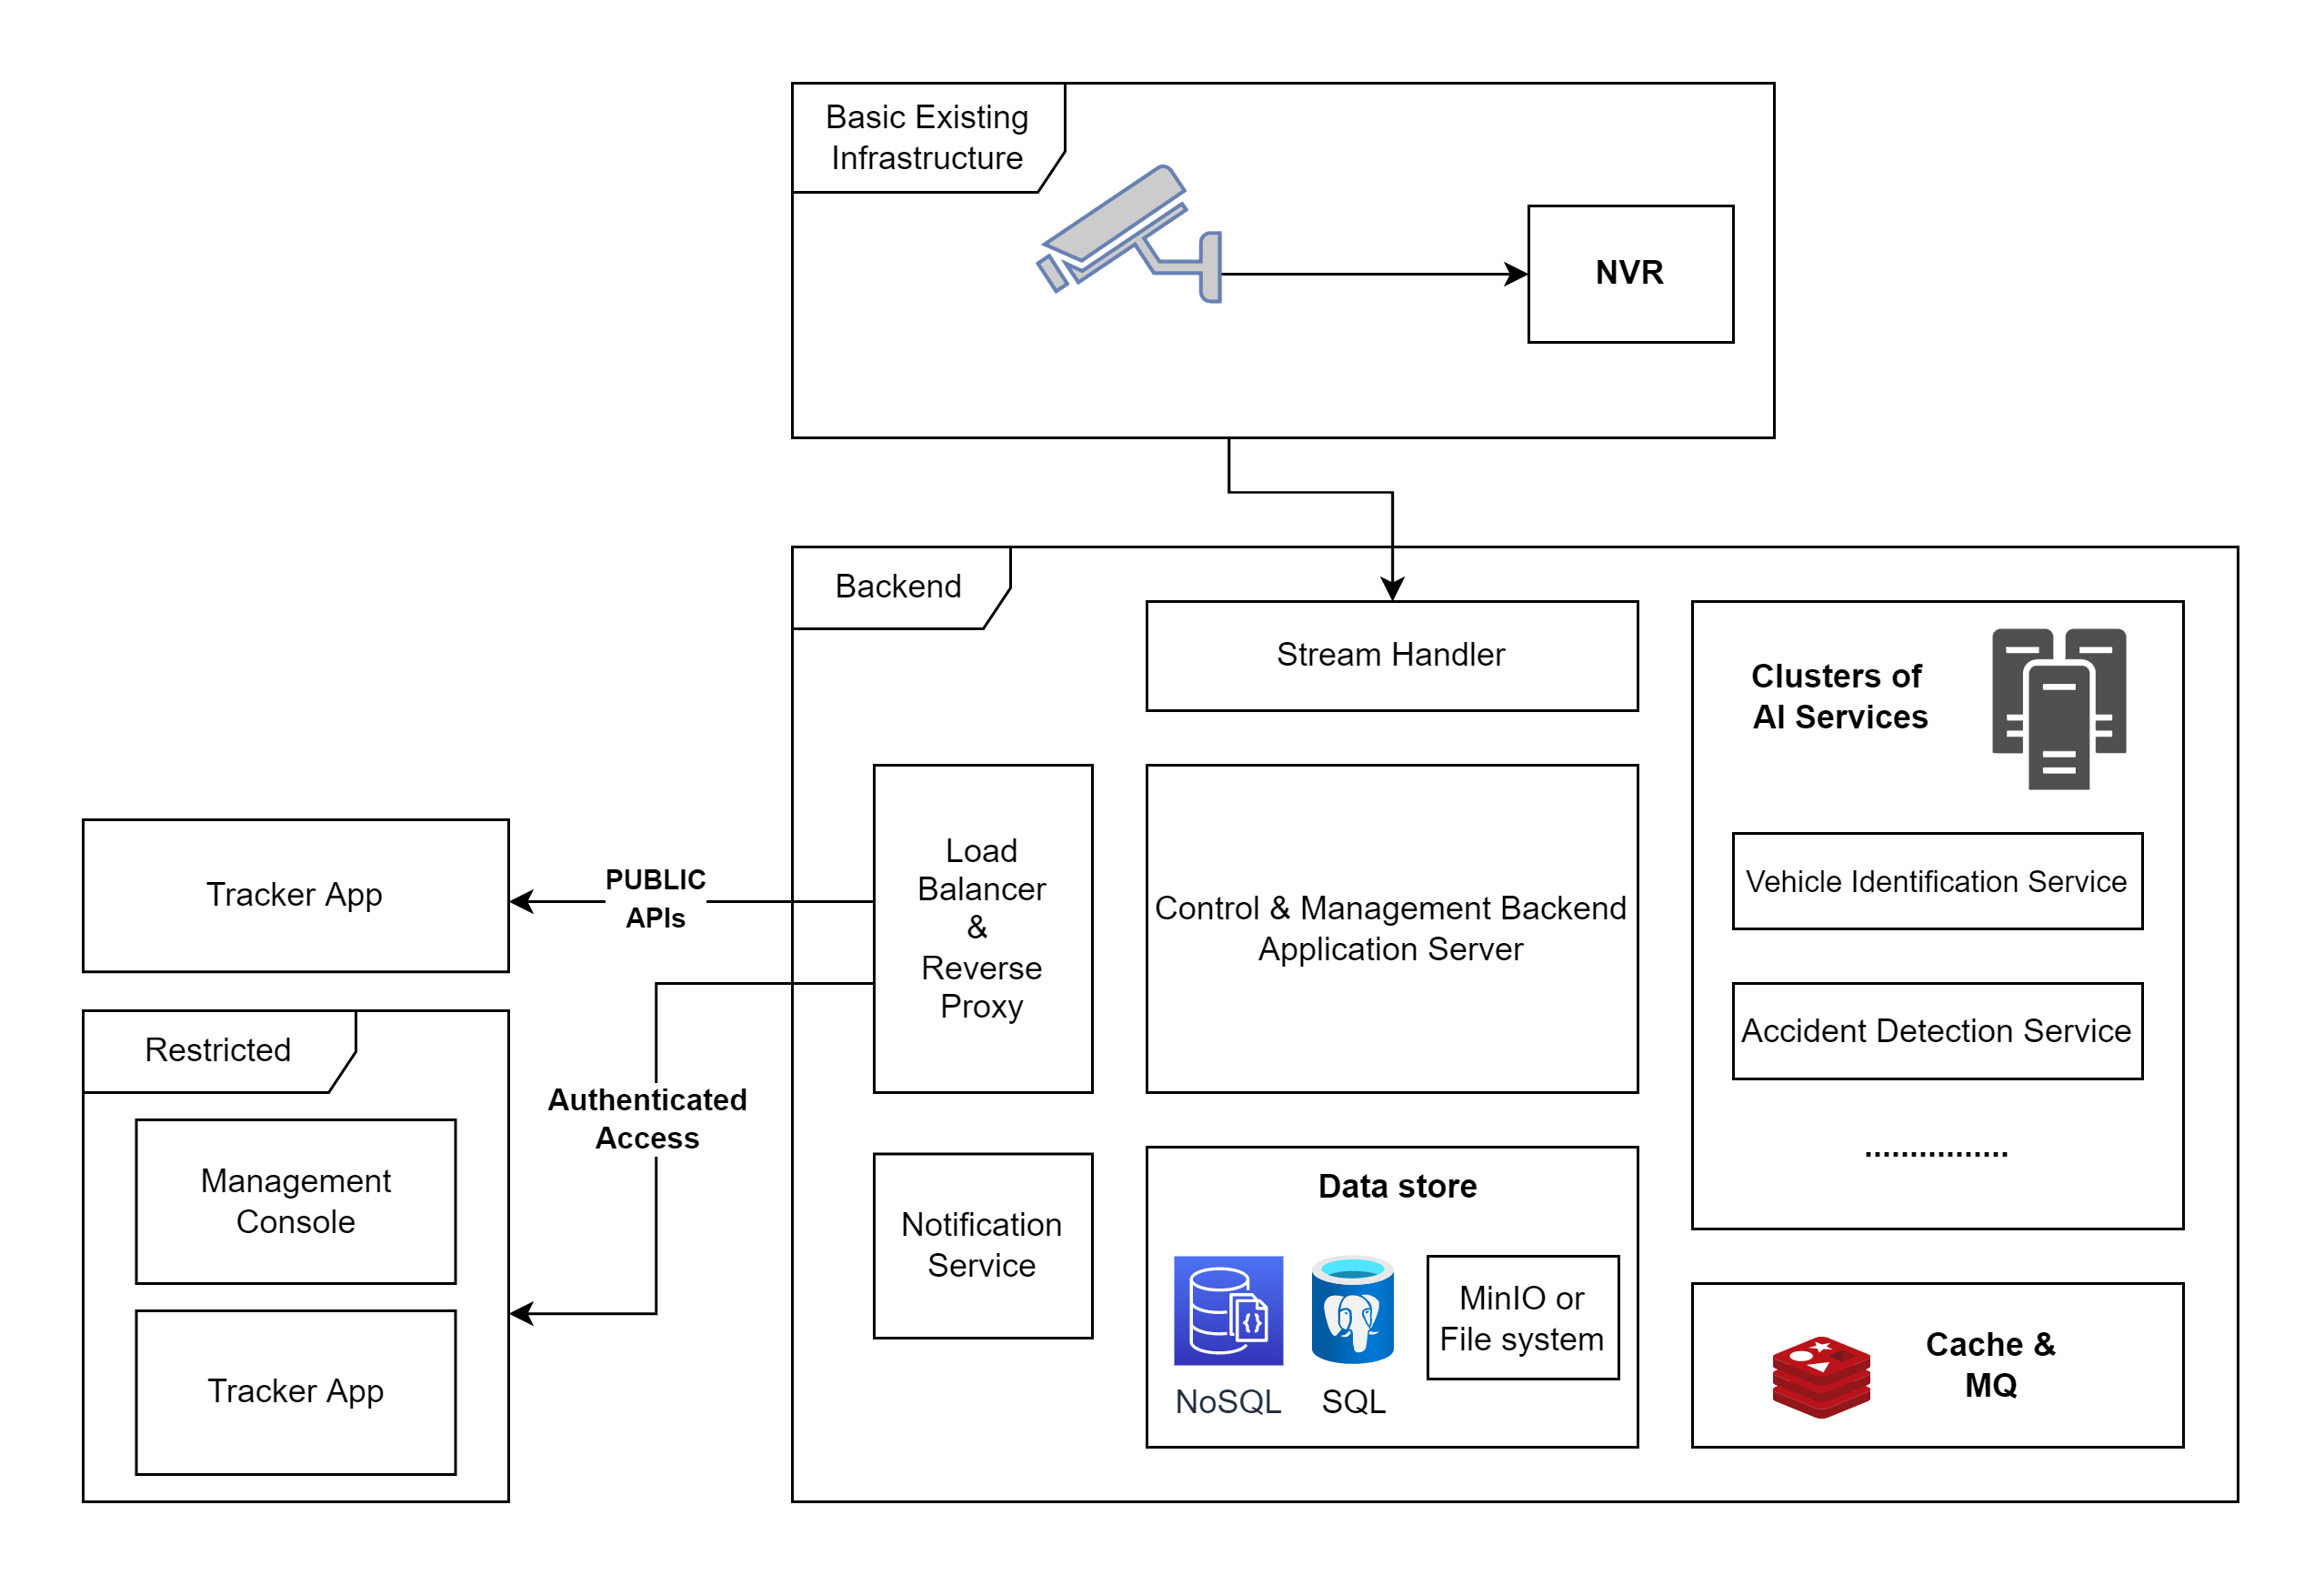
\includegraphics[width=\linewidth]{res/architecture_high_level}
		\end{center}
	\end{frame}

	\begin{frame}{Pipeline1}
		\begin{center}
			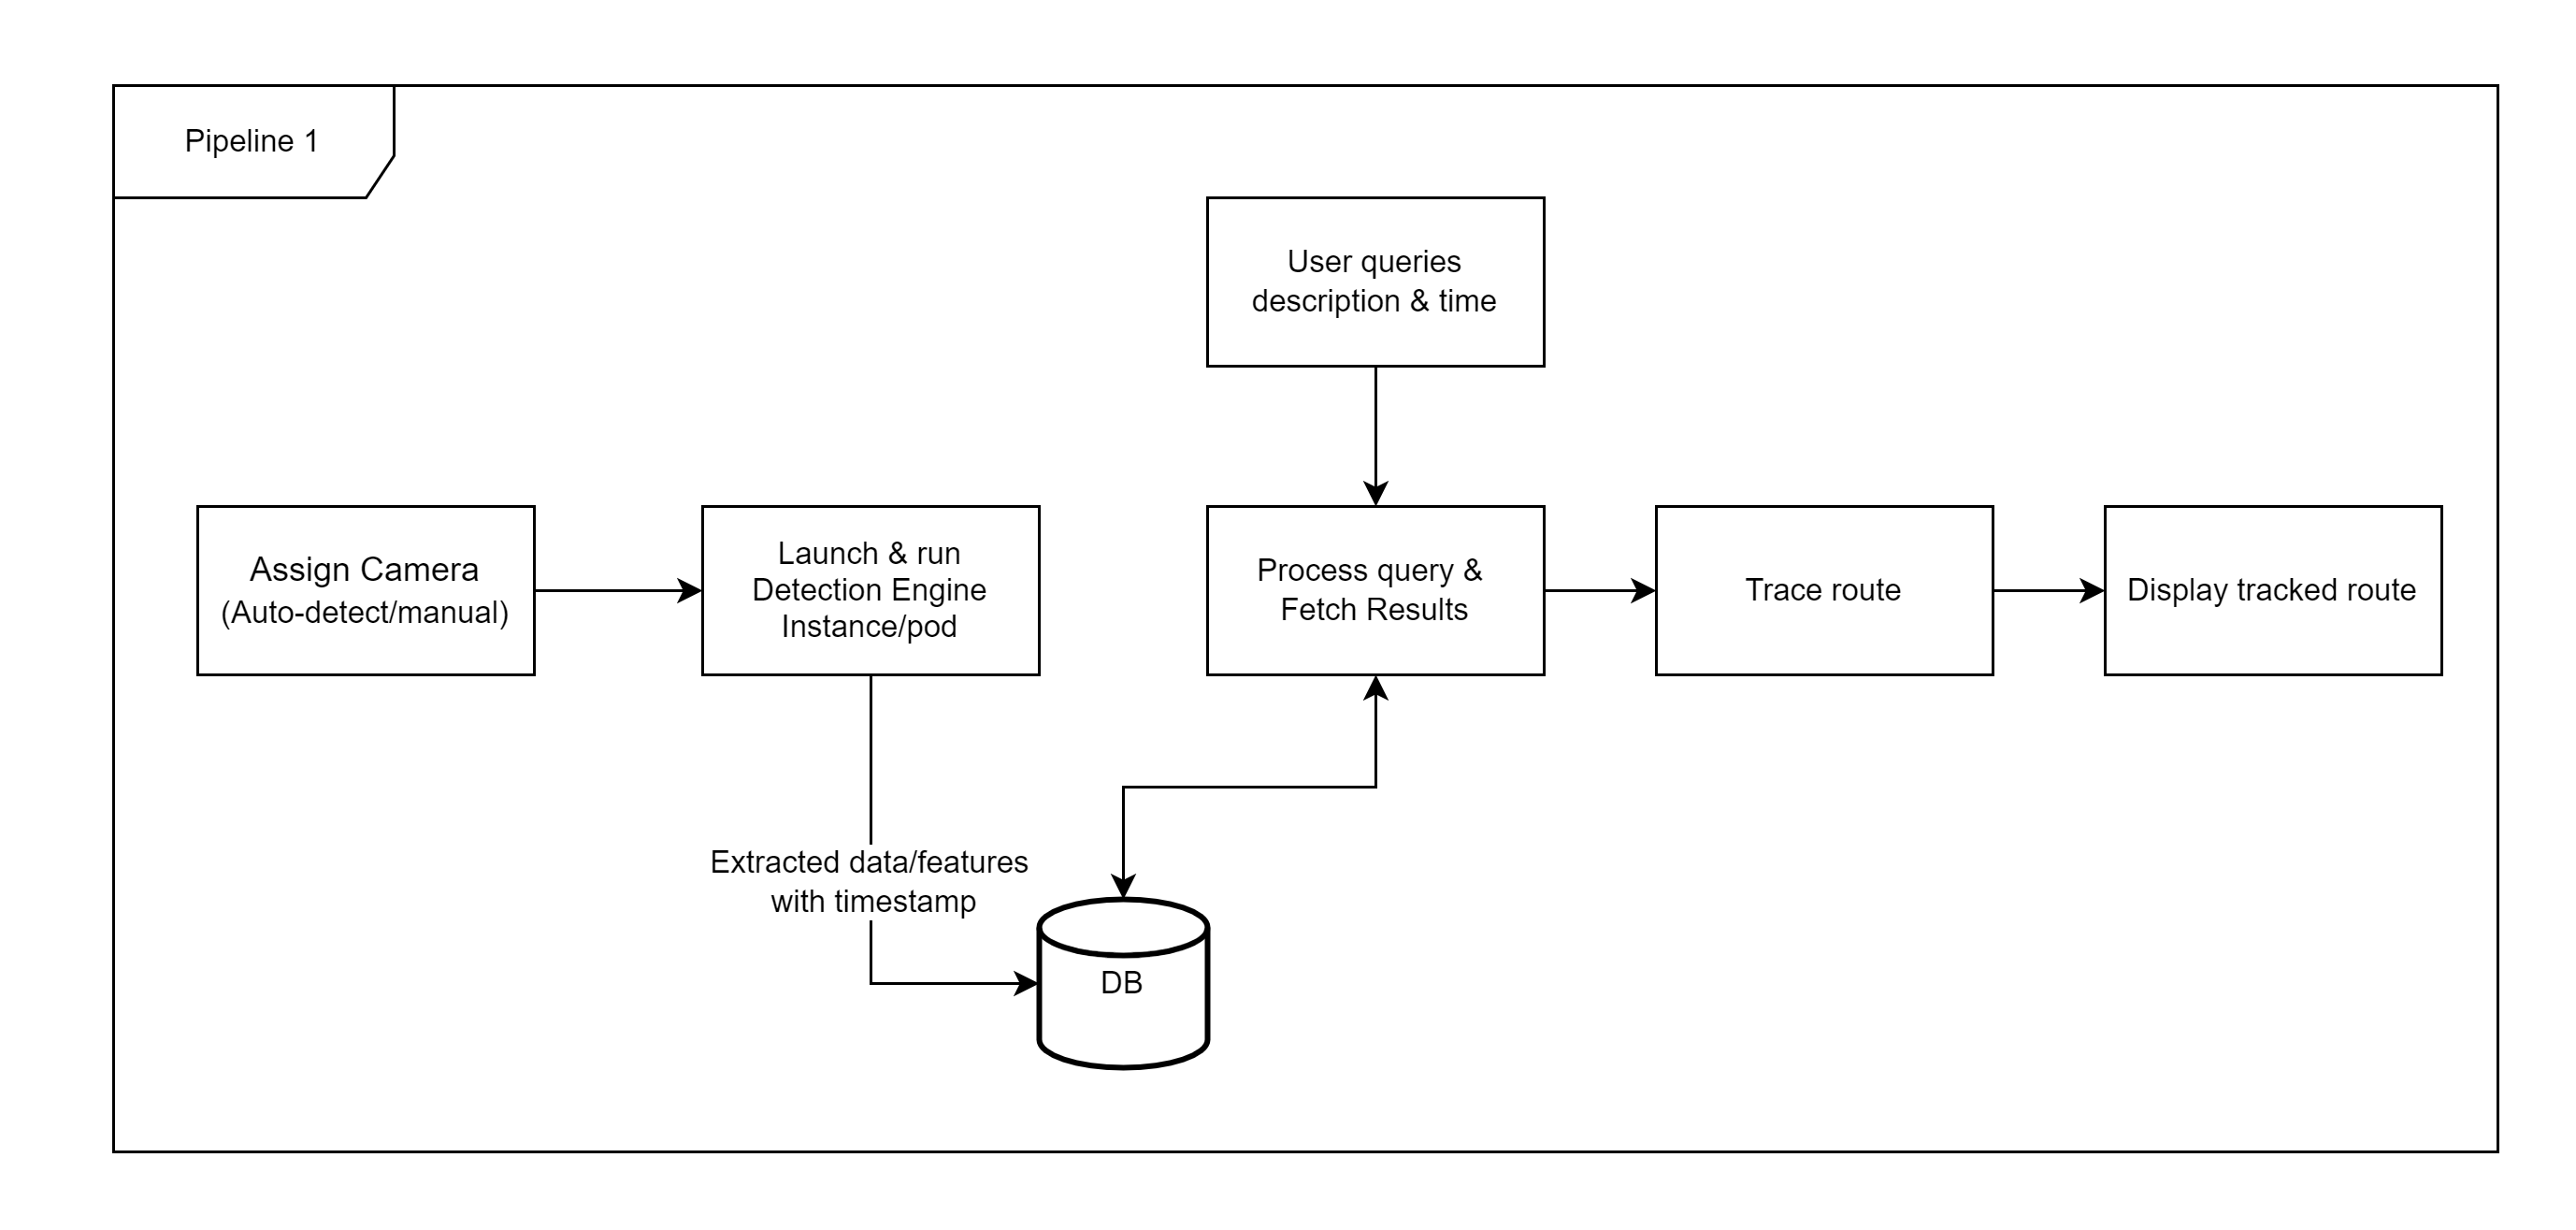
\includegraphics[width=\linewidth]{res/pipeline1}
		\end{center}
	\end{frame}

	\begin{frame}{Pipeline2}
		\begin{center}
			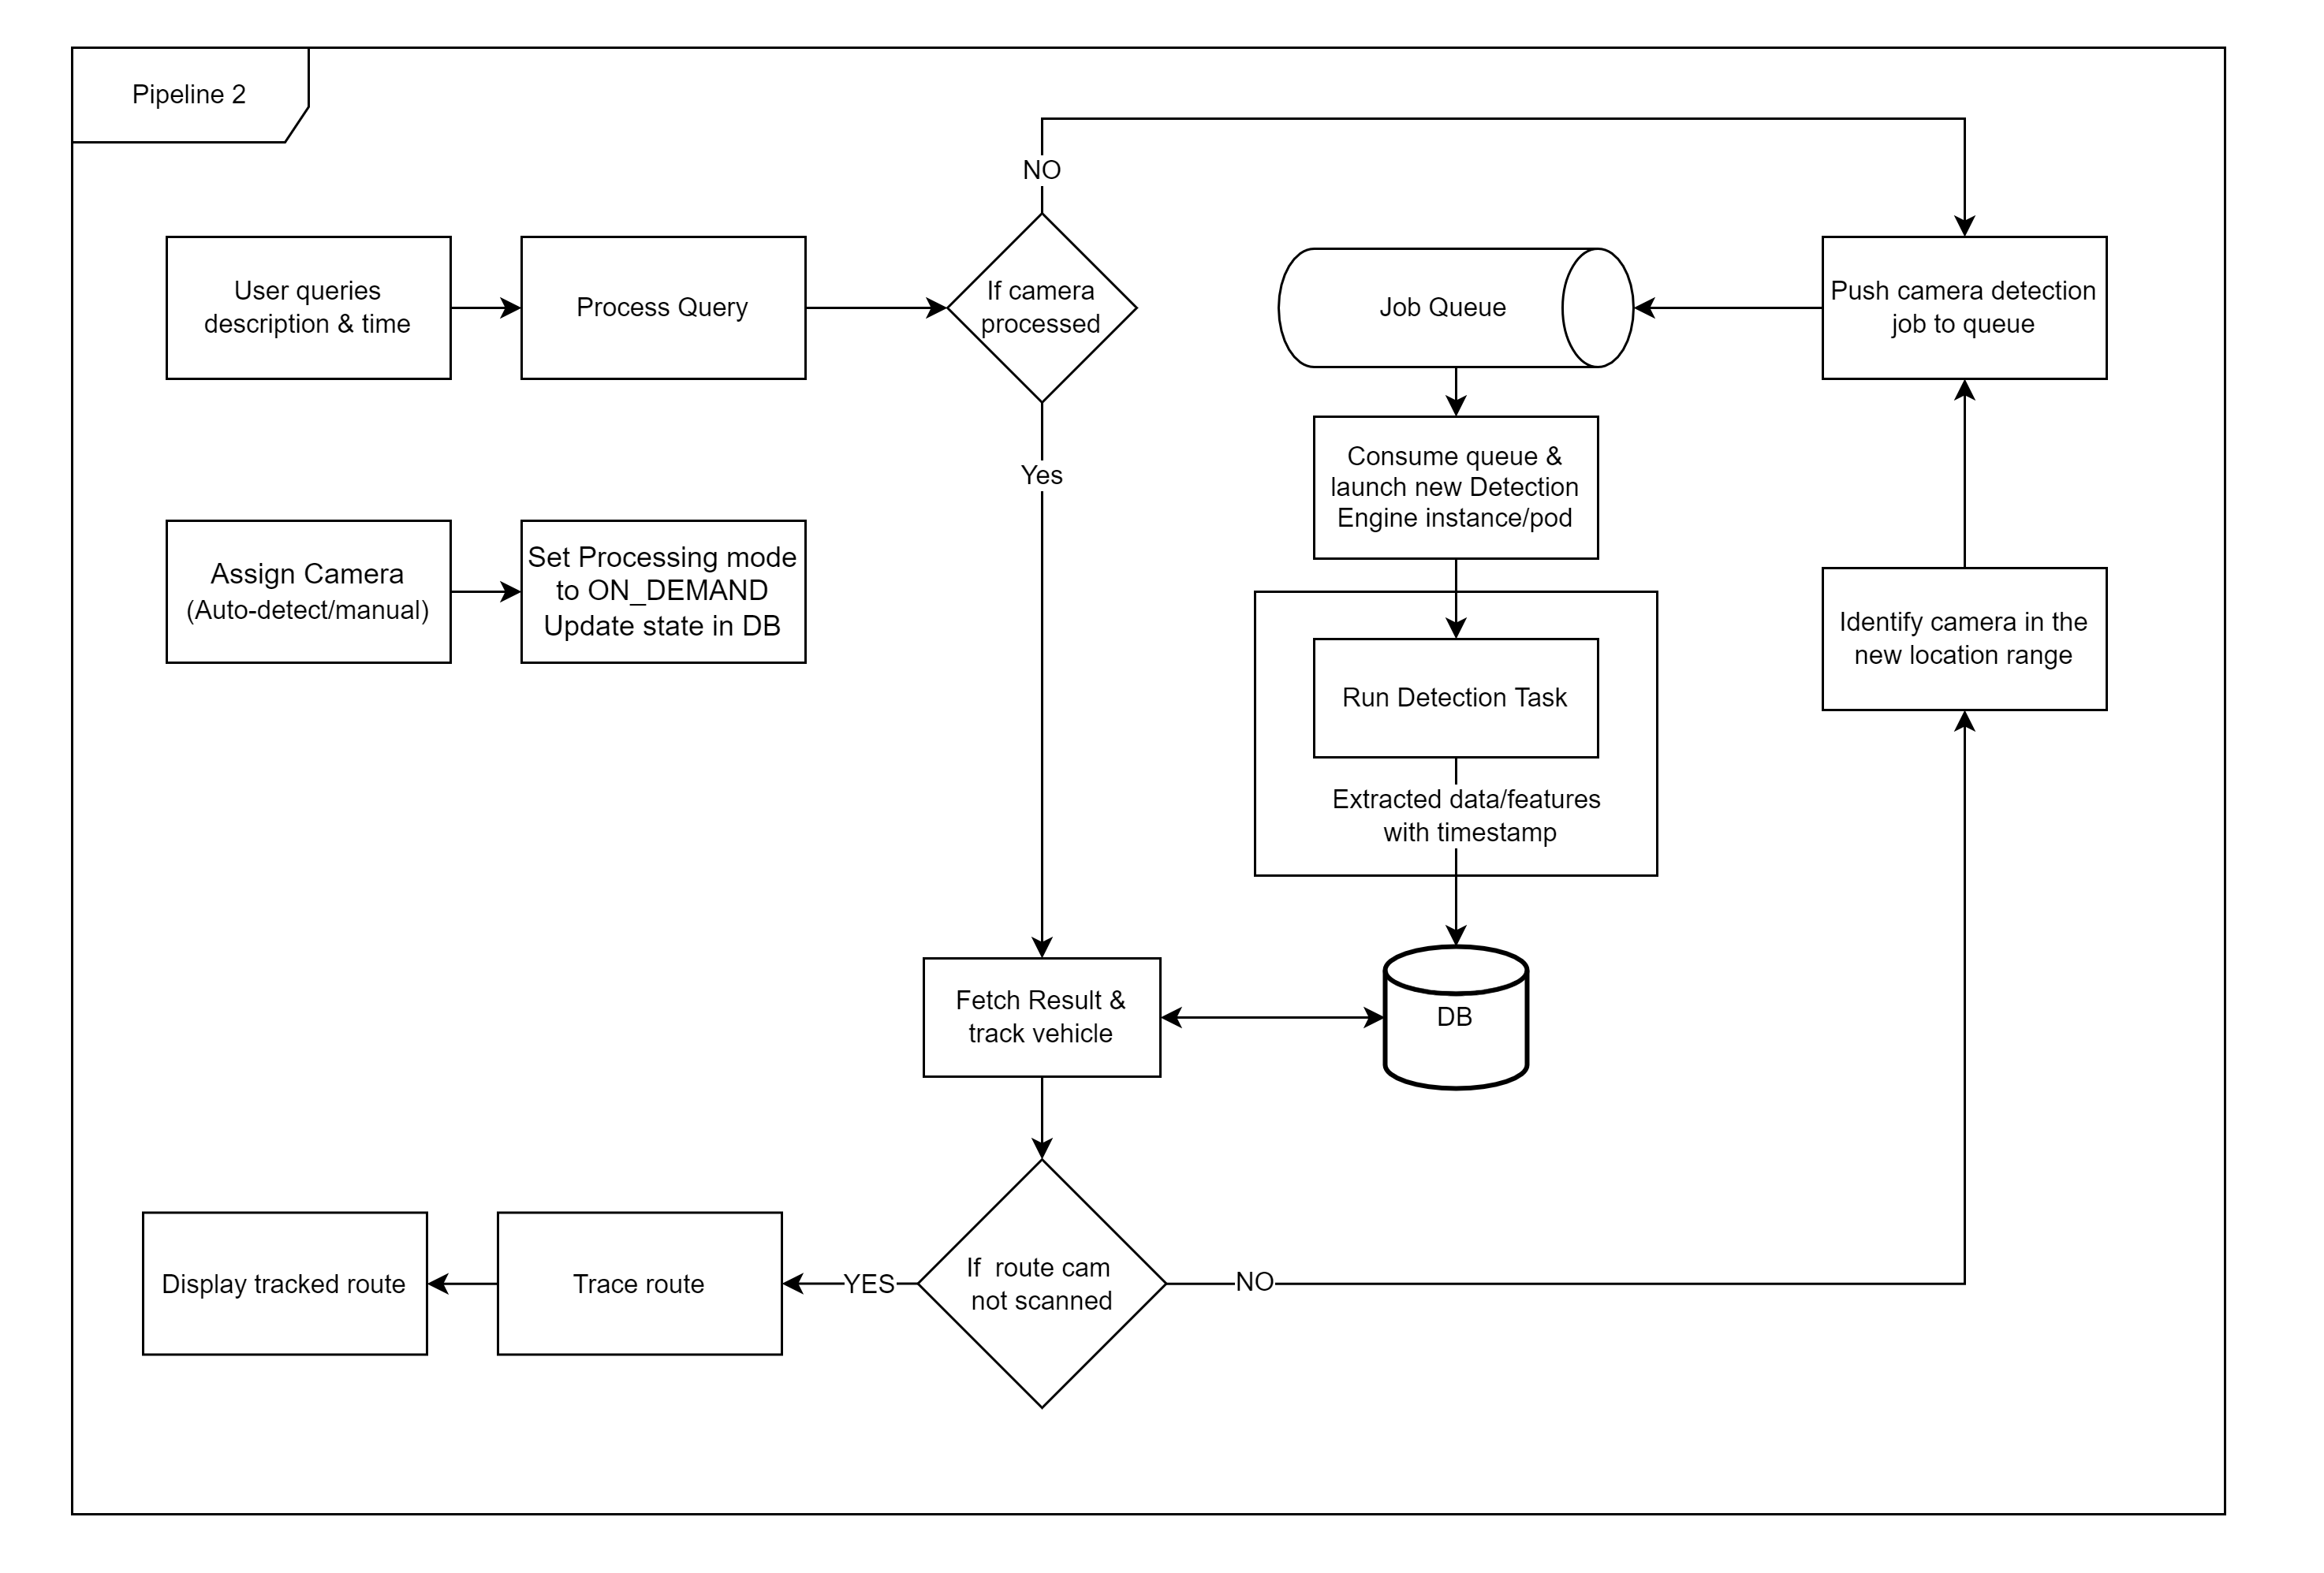
\includegraphics[width=\linewidth]{res/pipeline2}
		\end{center}
	\end{frame}


	%---------------------------------------------------------------------------
	% WORKS DONE SO FAR --------------------------------------------------------
	%---------------------------------------------------------------------------

	\section{Works done so far}
	\begin{frame}{Past works}
		\begin{center}
			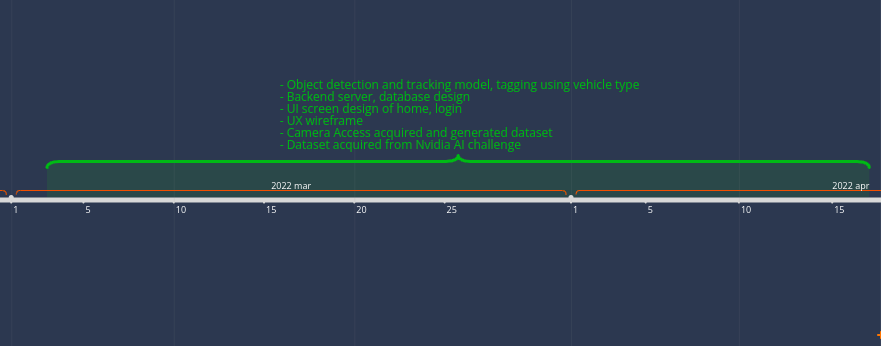
\includegraphics[width=1\linewidth]{res/timeline_old}
		\end{center}
		
	\end{frame}
	\subsection{AI model}
	\begin{frame}{Experimented with Classical Object detection methods}
		\begin{itemize}
			\item K-Means algorithm used for color extraction
				\link{https://github.com/Project-Dragon-Fly/tutorial-trials/blob/tutorial\_testing/Color\%20detection.ipynb}{notebook}
			
			\item Using OpenCV to detect object  
				\link{https://github.com/Project-Dragon-Fly/tutorial-trials/blob/tutorial\_testing/OpenCV-image-difference.ipynb}{notebook} $|$ 
				\link{https://drive.google.com/file/d/1-2EAoUBxMzfnMO3tVJFJ0qvGnXMFp4zL/view}{video}
			
			\item Harr algorithm to detect Bus and Car
				\link{https://github.com/Project-Dragon-Fly/tutorial-trials/blob/tutorial\_testing/OpenCV\%20-\%20Haar\%20algo.ipynb}{notebook} $|$
				\link{https://drive.google.com/file/d/1XYbVf6I2ZJSSdO2SsZECK9rNoYQwROM9/view}{video}
		\end{itemize}
		\begin{small}
			Video are generated using the code mentioned in this \link{https://github.com/Project-Dragon-Fly/tutorial-trials/blob/tutorial\_testing/Detection\_video\_generator.ipynb}{notebook}
		\end{small}
	\end{frame}

	\begin{frame}{Exploring various AI methods}
		\begin{itemize}
			\item Several YouTube tutorials and web articles are referenced to get understanding of AI methods and its evolution, which are summarized in this \link{https://docs.google.com/presentation/d/1ugCdqNADQ1QNd91lMP4BmbFBKYhkMoDrN2yIf\_t7SkI/edit?usp=sharing}{google slides}.
			
			\item Tensorflow provided this \link{https://github.com/Project-Dragon-Fly/tutorial-trials/blob/tutorial\_testing/object\_detection\_tensorflow\_tutorial.ipynb}{notebook} showing the usage of mobile-ssd/f-rcnn to detect general objects.
			
			\item Followed through the beginners tutorial provided by Tensorflow Team, saved at \link{https://github.com/Project-Dragon-Fly/tutorial-trials/tree/tutorial\_testing/YouTube\%20Tutorial\%20-\%20TensorFlow}{github}.
			\begin{itemize}
				\item Emphasis on working of CNN
				\item Got at glance at intermediate layer output of horse-human classifier. Output saved at  \link{https://github.com/Project-Dragon-Fly/tutorial-trials/blob/tutorial\_testing/YouTube\%20Tutorial\%20-\%20TensorFlow/Tutorial\%204\%20-\%20CNN\%20on\%20complex\%20images.ipynb}{notebook}
			\end{itemize}
		\end{itemize}
	\end{frame}

	\begin{frame}[allowframebreaks]{Notable GitHub repository}
		\begin{itemize}
			\item The official \link{https://github.com/ahmetozlu/tensorflow\_object\_counting\_api}{TensorFlow object counting api}. Houses various models (TensorFlow Model garden), tutorial notebooks. 
			
			\item The \link{https://github.com/taipingeric/yolo-v4-tf.keras}{taipingeric/yolo-v4-tf.keras} trained in YOLOv4, keras implementation. \link{https://github.com/Project-Dragon-Fly/tutorial-trials/blob/tutorial\_testing/Colab/YOLO-v4-tf-keras.ipynb}{notebook} $|$ \link{https://drive.google.com/file/d/16xsOZQjN-lKYAu7g7dlDvQIyyQhyfaBk/view?usp=sharing}{video1} $|$
			\link{https://drive.google.com/file/d/1ANPDVv4ZV2bVCmAM9H7SVpTrf3Pj9CIf/view?usp=sharing}{video2} $|$
			\link{https://drive.google.com/file/d/1-6vzo6-AmHlTGrR0W20heivqQ1uCJUQe/view?usp=sharing}{video3}
			
			\item Object Detection toolkit based on \link{https://github.com/PaddlePaddle/PaddleDetection}{PaddlePaddle}. It supports object detection, instance segmentation, multiple object tracking and real-time multi-person keypoint detection.
			
			\item Object Detection and Multi-Object Tracking by \link{https://github.com/yehengchen/Object-Detection-and-Tracking}{yehengchen}
			
			\break
			\item The \link{https://github.com/theAIGuysCode/yolov4-deepsort.git}{theAIGuysCode} uses 
			\begin{itemize}
				\item \textbf{YOLO model} to detect vehicles
				\item \textbf{deep-sort} model to track movement
			\end{itemize}
			Few observations
			\begin{itemize}
				\item Real-time speed achieved
				\item Implemented in python - TensorFlow
				\item Tracking is not accurate - affected by object occlusion, accuracy of YOLO, near identical objects, closely spaced objects, sudden non-linear movement.
			\end{itemize}
			Tried-out the repo \link{https://github.com/Project-Dragon-Fly/tutorial-trials/blob/tutorial\_testing/Colab/obj\%20detection\%20and\%20tracking.ipynb}{notebook} $|$ \link{https://drive.google.com/file/d/172r\_jCelsVzNxqjhgWjvTbXkcNGTN4Yl/view?usp=sharing}{video1} $|$ \link{https://drive.google.com/file/d/1EwC8sfuPR-gbwt8udMf6tlxATn6Ud3oA/view?usp=sharing}{video2} $|$
			\link{https://drive.google.com/file/d/1-4hTbPk6xC-Cb58G2ZXE6qi6WpWuD-XT/view?usp=sharing}{video3}	
		\end{itemize}
	\end{frame}

	\begin{frame}{Building custom YOLOv4 model}
		\framesubtitle{Model Information}
		See code at \link{https://github.com/Project-Dragon-Fly/tutorial-trials/blob/tutorial\_testing/Colab/indian\_vehicle\_detection.ipynb}{notebook}
		\begin{table}[]
			\centering
			\resizebox{\textwidth}{!}{%
				\begin{tabular}{|l|l|}
					\hline
					Framework used            & DarkNet                  \\ \hline
					Initial weight            & official 80 class weight \\ \hline
					Target classes            & 9                        \\ \hline
					Platform for training     & Google Colab             \\ \hline
					Current mAP               & 96.7 \%                  \\ \hline
					Current Iterations        & 4800                     \\ \hline
					DataSet & \begin{tabular}[c]{@{}l@{}}500 till 2800 iteration\\ 733 after wards\end{tabular} \\ \hline
					Approx Hrs Spent training & 25-30 hrs                \\ \hline
				\end{tabular}%
			}
		\end{table}
	\end{frame}

	\begin{frame}[allowframebreaks]{Building custom YOLOv4 model}
		\framesubtitle{Current Model evaluation}
		\begin{center}
			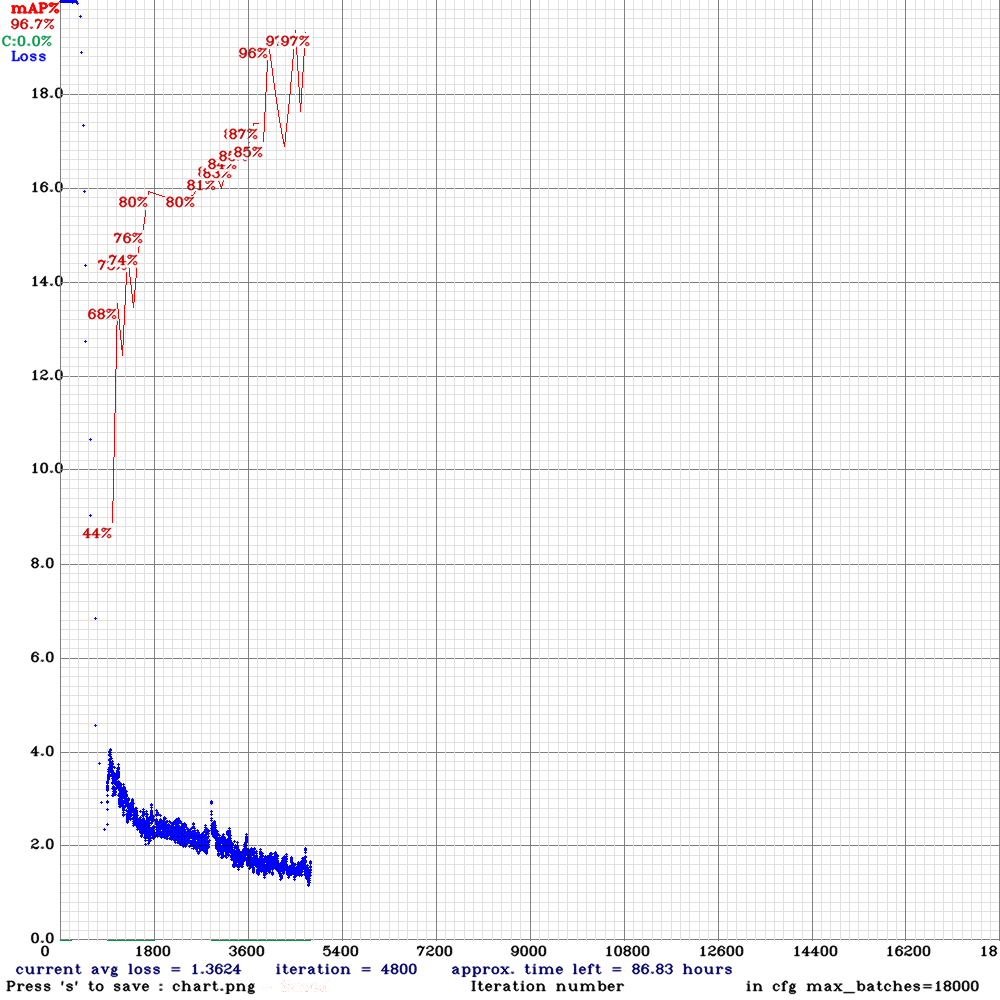
\includegraphics[height=0.7\textheight]{res/darknet_training_chart}
		\end{center}
	
		\newpage
		\begin{scriptsize}
			detections\_count = 7729, unique\_truth\_count = 1956  \\ 
			class\_id = 0, name = auto, ap = 97.27\%   	 (TP = 285, FP = 15) \\
			class\_id = 1, name = bus, ap = 99.76\%   	 (TP = 217, FP = 10) \\
			class\_id = 2, name = tempo traveller, ap = 96.50\%   	 (TP = 57, FP = 3) \\
			class\_id = 3, name = tractor, ap = 98.93\%   	 (TP = 131, FP = 1) \\
			class\_id = 4, name = truck, ap = 99.20\%   	 (TP = 346, FP = 36) \\
			class\_id = 5, name = van, ap = 96.71\%   	 (TP = 98, FP = 21) \\
			class\_id = 6, name = two wheeler, ap = 88.59\%   	 (TP = 480, FP = 104) \\
			class\_id = 7, name = car, ap = 93.92\%   	 (TP = 216, FP = 39) \\
			class\_id = 8, name = jcb, ap = 100.00\%   	 (TP = 0, FP = 0) \\
			
			for conf\_thresh = 0.25, precision = 0.89, recall = 0.94, F1-score = 0.91  \\
			for conf\_thresh = 0.25, TP = 1830, FP = 229, FN = 126, average IoU = 72.94 \%  \
			
			IoU threshold = 50 \%, used Area-Under-Curve for each unique Recall  \\
			mean average precision (mAP@0.50) = 0.967638, or 96.76 \% \\
			Total Detection Time: 268 Seconds
		\end{scriptsize}		
		\newpage
		
		\begin{center}
			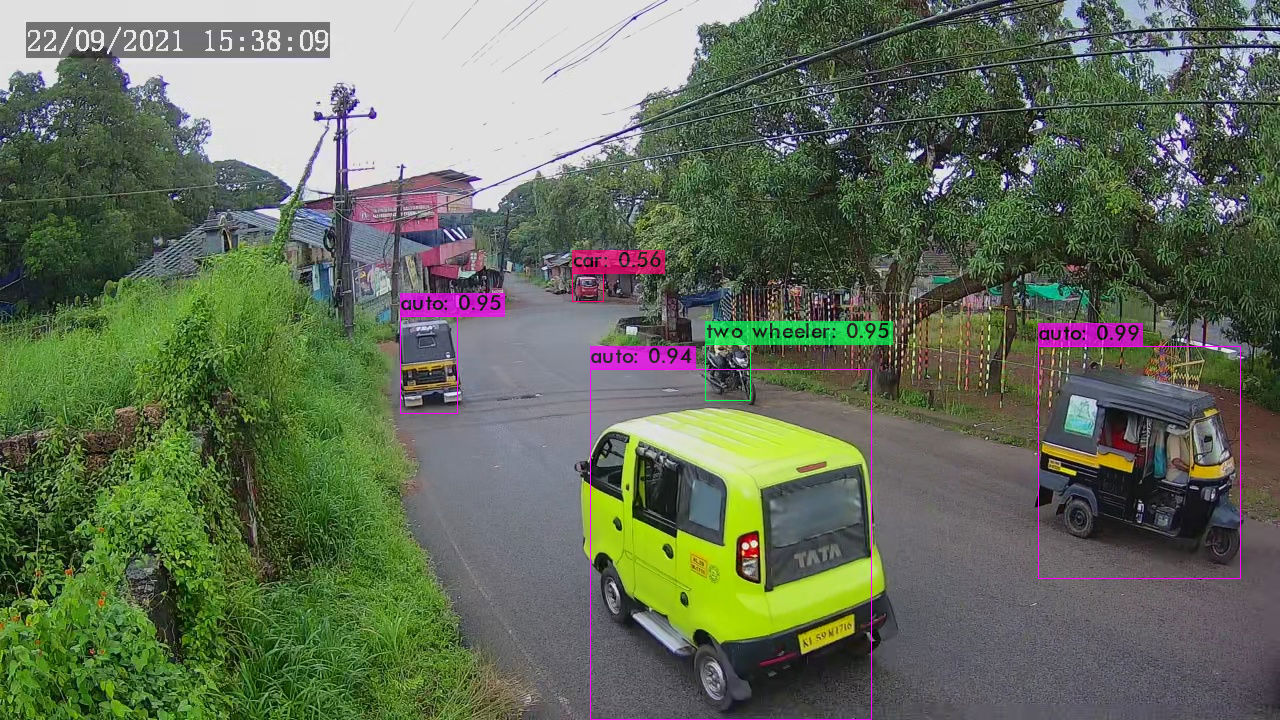
\includegraphics[width=\linewidth]{res/data_set1/predictions}
		\end{center}
	\end{frame}


	\begin{frame}[allowframebreaks]{Building custom YOLOv4 model}
		\framesubtitle{Dataset information (from internet)}
		Fetched from \link{https://www.kaggle.com/datasets/dataclusterlabs/indian-vehicle-dataset}{Kaggle}. Used labelImg to label images. 
		\begin{table}[]
			\centering
			\begin{tabular}{|l|l|}
				\hline
				\textbf{Frequency}    & \textbf{Label Name} \\ \hline
				557                   & two wheeler         \\ \hline
				354                   & truck               \\ \hline
				297                   & auto                \\ \hline
				233                   & car                 \\ \hline
				220                   & bus                 \\ \hline
				133                   & tractor             \\ \hline
				101                   & van                 \\ \hline
				1                     & jcb                 \\ \hline
				\textbf{Total Boxes}  & \textbf{1956}       \\ \hline
				\textbf{Total Images} & \textbf{733}        \\ \hline
			\end{tabular}
		\end{table}
		
		
		
		\newpage
		\begin{figure}
			\includegraphics[width=0.24\linewidth]{"res/data_set1/image1"} \hfill
			\includegraphics[width=0.24\linewidth]{"res/data_set1/image2"} \hfill
			\includegraphics[width=0.24\linewidth]{"res/data_set1/image3"} \hfill
			\includegraphics[width=0.24\linewidth]{"res/data_set1/image4"}
		\end{figure}
	\end{frame}


	\begin{frame}[allowframebreaks]{Building custom YOLOv4 model}
		\framesubtitle{Dataset information (from camera network)}
		Fetched from camera infrastructure. Used labelImg to label images.
		\begin{center}
			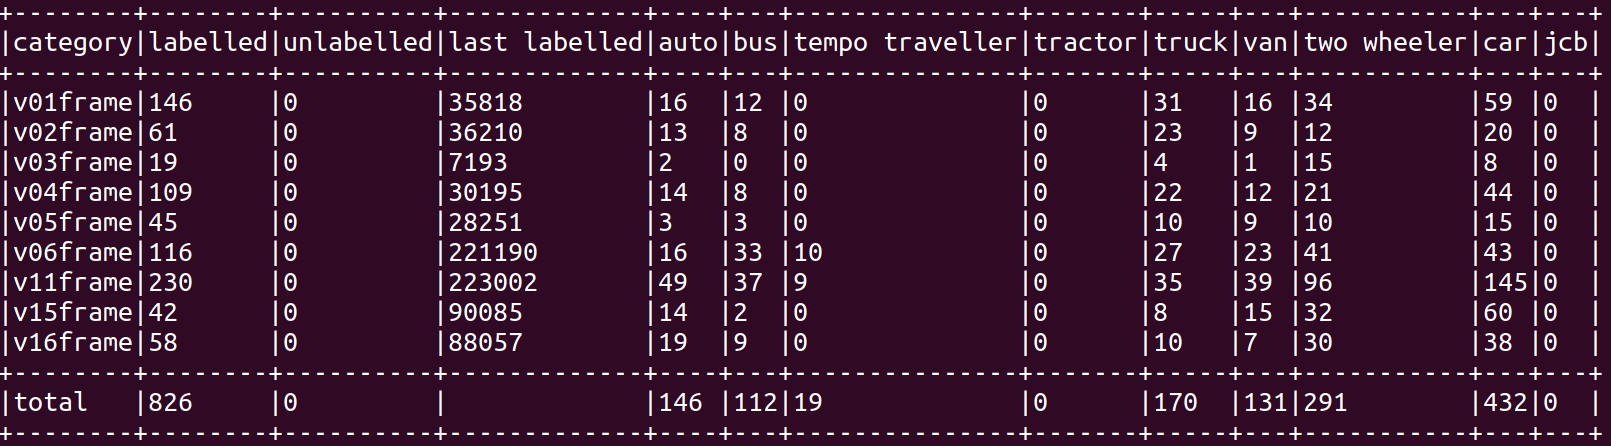
\includegraphics[width=\linewidth]{res/data_set2/custom_label_stat}
		\end{center}
		
		\newpage
		\begin{figure}
			\includegraphics[width=0.48\linewidth]{"res/data_set2/image1"} \hfill
			\includegraphics[width=0.48\linewidth]{"res/data_set2/image2"}
			\\[\smallskipamount]
			\includegraphics[width=0.48\linewidth]{"res/data_set2/image3"} \hfill
			\includegraphics[width=0.48\linewidth]{"res/data_set2/image4"}
		\end{figure}
	\end{frame}


	\subsection{UI/UX}	
	\begin{frame}{Login page}
		\begin{center}
			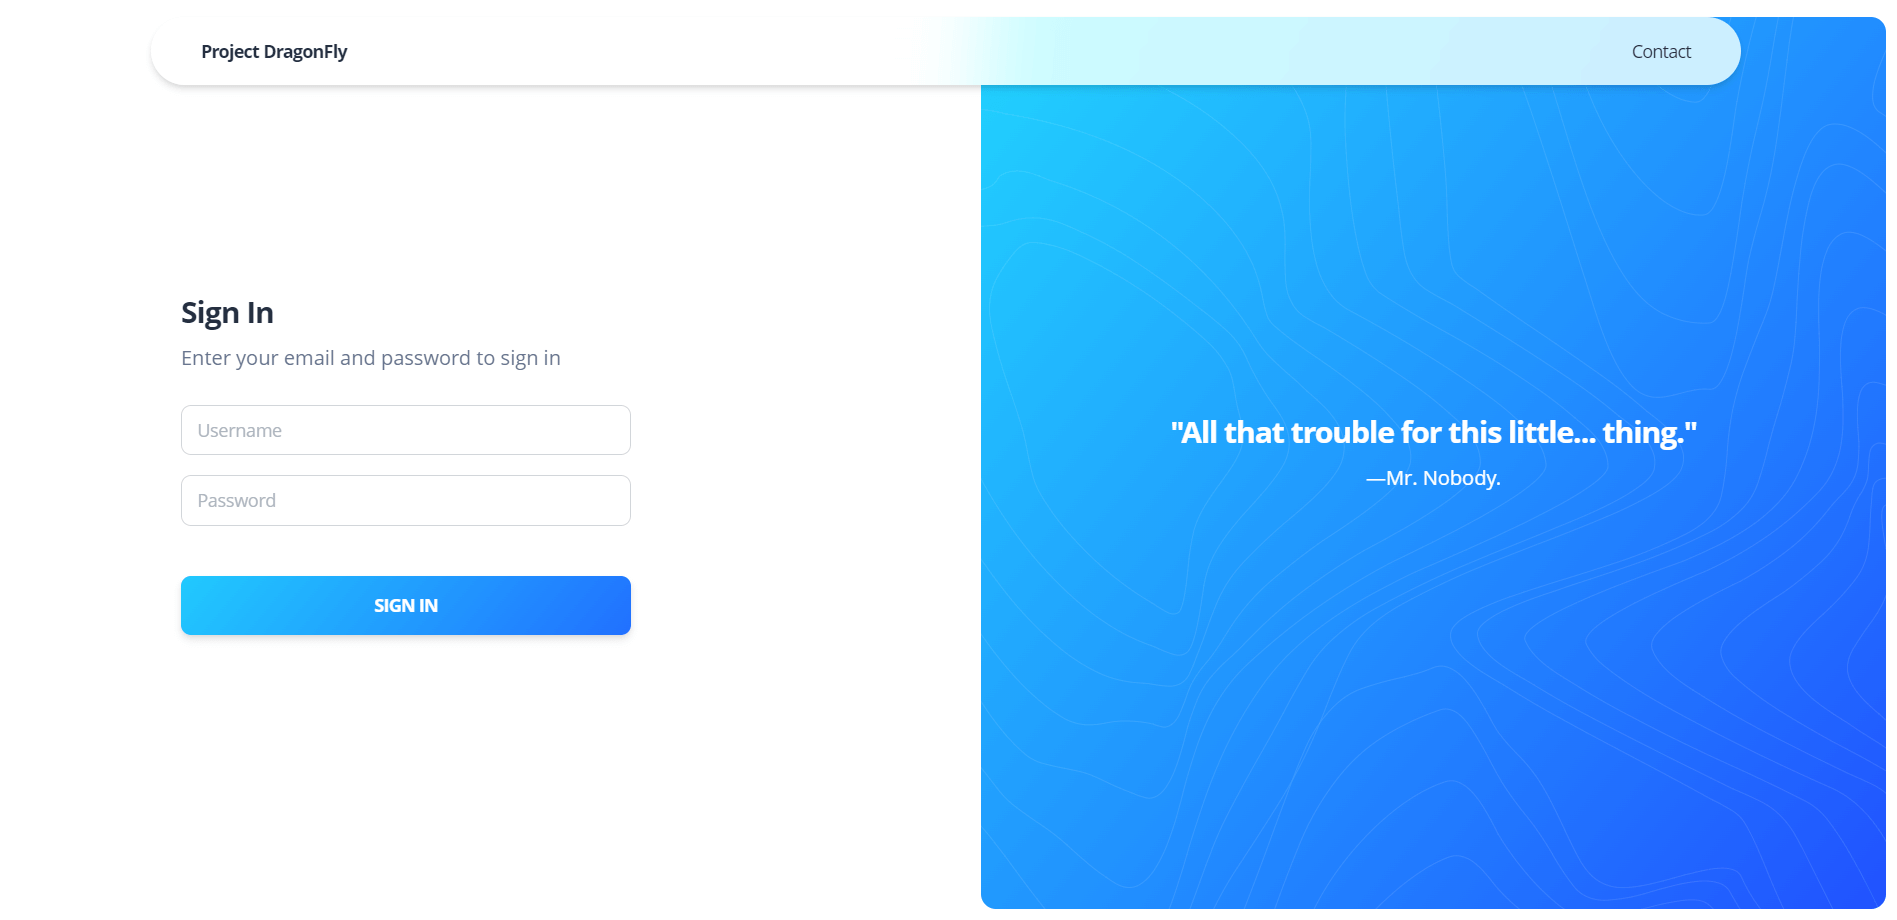
\includegraphics[width=1\linewidth]{res/loginpage}
		\end{center}
	\end{frame}

	\begin{frame}{Home page}
		\begin{center}
			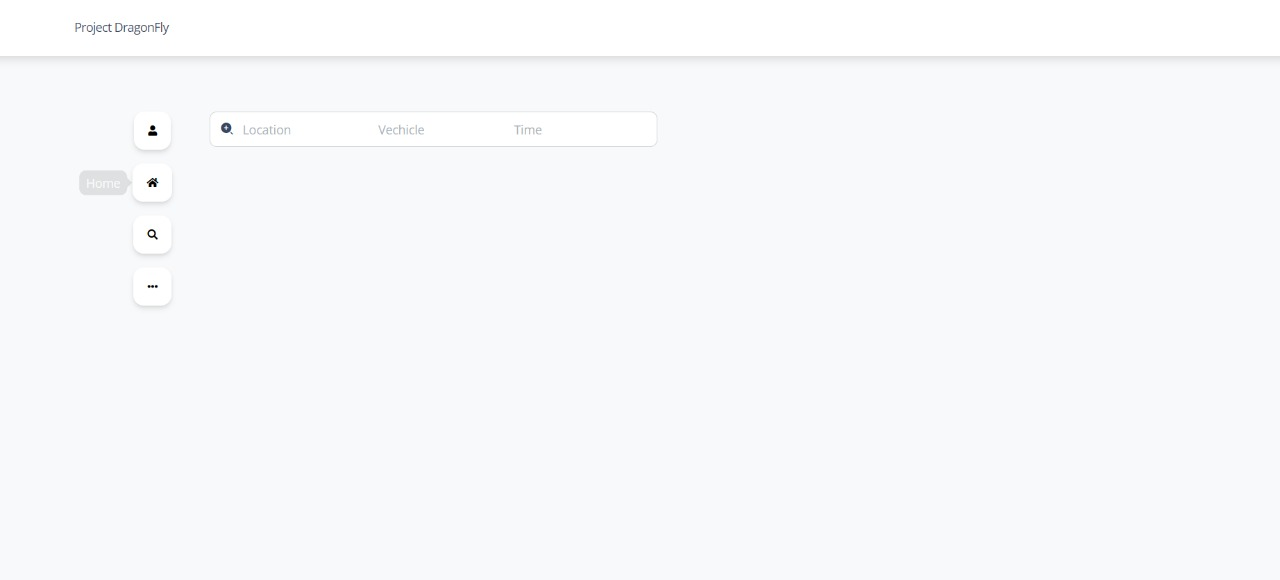
\includegraphics[width=1\linewidth]{res/homepage}
		\end{center}
	\end{frame}

	\subsection{Other Updates}
	\begin{frame}{Works done : Other updates}
		\begin{itemize}
			\item Defining data format - laying structures \link{https://github.com/Project-Dragon-Fly/mock-servers/blob/main/data\_format.md}{visit here}
			\item Development of \link{https://github.com/Project-Dragon-Fly/backend-server}{boilerplate codes}
			\item Registered and acquired data from \link{https://www.aicitychallenge.org/}{NVIDIA AI City Challenge}
			\item Obtained access and checked streaming data from video frames.
			\item Exploring Google Maps API and Geo-Pandas.
		\end{itemize}
		\begin{center}
			\link{https://github.com/Project-Dragon-Fly}{GitHub Organization} $|$ \link{https://drive.google.
				com/drive/folders/1GbQ1L1mfY97nh3NXE4Iyz\_e2gIwvmH0V?usp=sharing}{Shared Google Drive}
		\end{center}
	\end{frame}

	%---------------------------------------------------------------------------
	% FUTURE WORKS PLANNED -----------------------------------------------------
	%---------------------------------------------------------------------------
	\section{Future Planned works}
	\begin{frame}[allowframebreaks]{Future Planned works}
		\begin{center}
			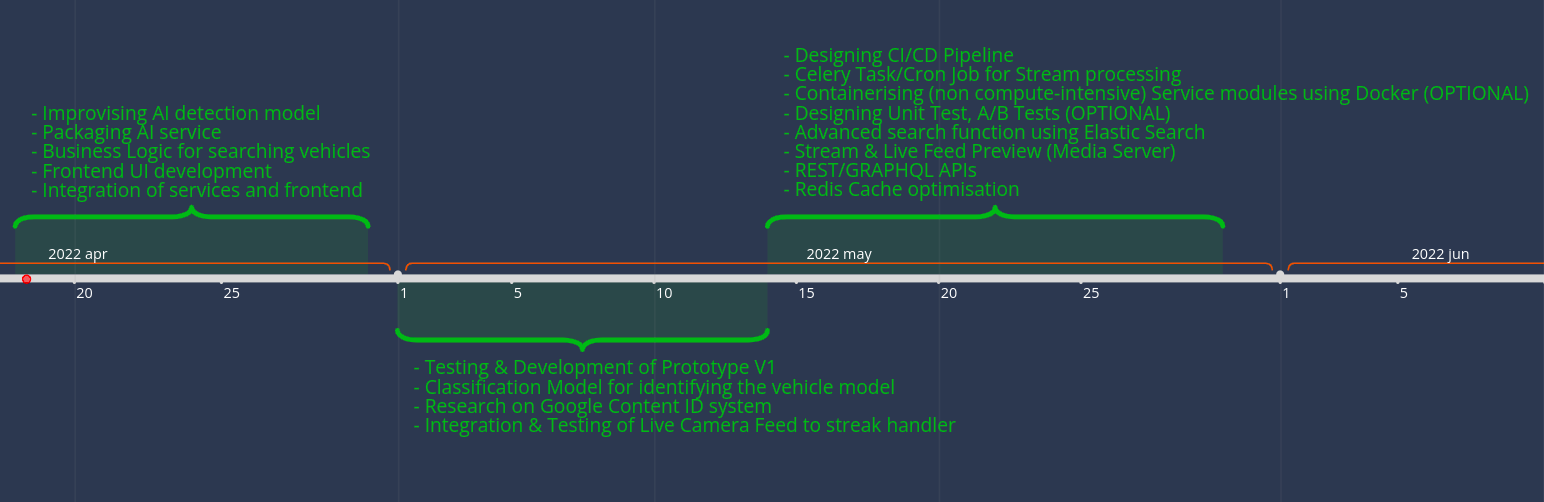
\includegraphics[width=1\linewidth]{res/time_line_future}
		\end{center}
		
		\begin{itemize}
			\item AI Model \\
			\begin{itemize}
				\item Packaging code as service module
				\item Labeling of more data from video streams.
				\item Detection of major classes are given first priority, then for sub-classes.
			\end{itemize}
			
			\item Frontend \& UI/UX\\
			\begin{itemize}
				\item Development of user interfaces for displaying results, homepage, route map.
				\item Integration of Maps API
			\end{itemize}
		
			\item Back-end service\\
			\begin{itemize}
				\item Redefining Database relationship between various camera configuration needs to be properly defined.
				\item Business Logics for search and display
				\item Research on Route prediction algorithm \& Graph Database
				\item Integration of AI service for PoC Development
			\end{itemize}
		\end{itemize}
	\end{frame}

\end{document} 